\chapter{Elementos do texto}
\label{cap:texto}

% - - - - - - - - - - - - - - - - - - - - - - - - - - - - - - - - - - -
\section{Figuras}
\label{sec:figs} 
Rótulos de figuras e tabelas devem ser centralizados se tiverem até uma linha (Figura~\ref{fig:exemploFig1}), caso contrário devem estar justificados e identados em ambas as margens, como mostrado na Figura ~\ref{fig:exemploFig2}. Essa formatação já é realizada automaticamente pela classe \textsf{inf-ufg}.

Os compiladores \LaTeX\ provêem um mecanismo bastante simples para inclusão de figuras, o que pode ser feito com o auxílio de várias classes auxiliares (as mais comuns são \verb|graphic| e \verb|graphicx|). A classe \verb|inf-ufg| usa o comando \verb|\includegraphics|, da classe \verb|graphicx|, para a inclusão de figuras e não é necessário você colocar a extensão do arquivo neste comando. Por exemplo, para a figura \ref{fig:exemploFig1} os comandos usados foram:
\begin{Verbatim}
 \begin{figure}[htb]
  \centering
  
\includegraphics[width=0.40\textwidth]{fig/logo-ifg-vertical-goiania}
  \caption{Logo IFG.}
  \label{fig:exemploFig1}
 \end{figure}
 \fontefig{\cite{ifg2020}}
\end{Verbatim}


Ao se usar o compilador \LaTeX, as figuras podem estar nos formatos \textit{eps} e \textit{ps}. Ao se usar o PDF\LaTeX, as figuras podem estar nos formatos \textit{png}, \textit{jpg}, \textit{pdf} e \textit{mps}. A classe \verb|graphicx| também pode ser usada para a inclusão de figuras, nos formatos listados, ao se usar o PDF\LaTeX. Os comandos necessários são os mesmos ao se incluir figuras ao se usar o compilador \LaTeX. O uso do comando \verb|\includegraphics| faz com com que PDF\LaTeX\ procure primeiro por figuras com extensão \textit{pdf}, depois \textit{jpg}, depois \textit{mps} e por último \textit{png}. Aqui também não é necessário especificar a extensão do arquivo.

Para a inclusão das figuras \ref{fig:exemploFig1} à \ref{fig:exemploFig3} os comandos usados, tanto no \LaTeX\ quanto no PDF\LaTeX, seriam os mesmos. É claro que em cada caso devem estar disponíveis as figuras nos formatos suportados por cada compilador. Por exemplo, para a inclusão da figura \ref{fig:exemploFig3} foram usados:
\begin{Verbatim}
 \begin{figure}[!ht]
  \centering
  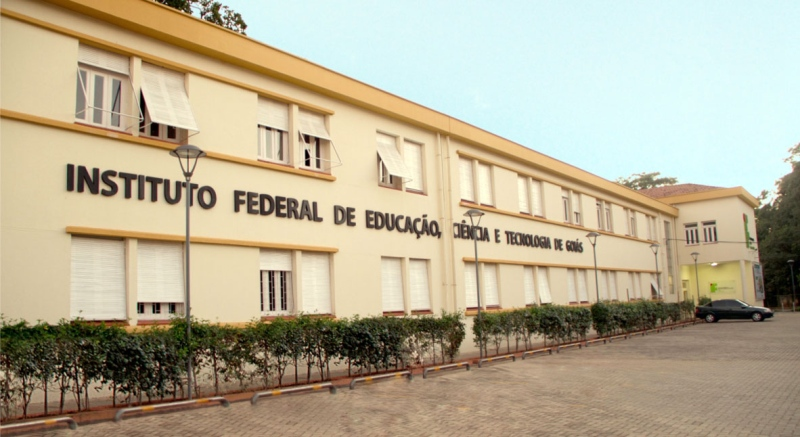
\includegraphics[width=0.40\textwidth]{./fig/foto-ifg}
  \caption{Câmpus Goiânia do IFG.}
  \label{fig:exemploFig3}
\end{figure}
\fontefig{\cite{ifg2020}}
\end{Verbatim}

\begin{figure}[!ht]
 \centering
  
\includegraphics[width=0.30\textwidth]{./fig/logo-ifg-vertical-goiania}
 \caption{Logo IFG.}
 \label{fig:exemploFig1}
\fontefig{\cite{ifg2020}}
\end{figure}

\begin{figure}[!ht]
 \centering
 
\includegraphics[width=0.60\textwidth]{./fig/logo-ifg}
 \caption{Esta figura é um exemplo de um rótulo de figura que ocupa mais de uma linha, devendo ser identado e justificado.}
 \label{fig:exemploFig2}
\fontefig{\cite{ifg2020}}
\end{figure}

\begin{figure}[H]
 \centering
  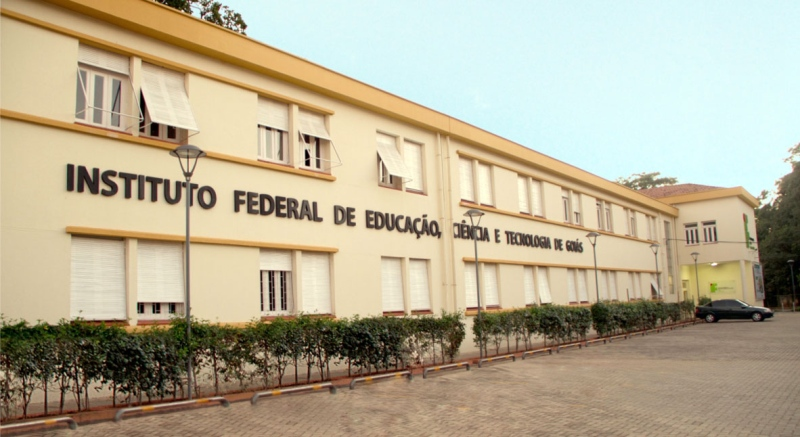
\includegraphics[width=0.70\textwidth]{./fig/foto-ifg}
  \caption{Câmpus Goiânia do IFG.}
 \label{fig:exemploFig3}
\fontefig{\cite{ifg2020}}
\end{figure}

\subsection{Subfiguras}
\label{subsec:subfigs} 
A classe \verb|subfigure| pode ser usada para a inclusão de figuras dentro de figuras (consulte a documentação da classe para maiores detalhes). Por exemplo, a Figura \ref{fig:subfiguras} contém duas subfiguras. Estas podem ser referencidas por rótulos independentes, ou seja, podem ser referenciadas como Figuras \ref{subfig:ex1} e \ref{subfig:ex2} ou Subfiguras \subref{subfig:ex1} e \subref{subfig:ex2}.
\begin{figure}[h]
 \centering
%   \subfigure[][Primeira subfigura.]
  \subfigure[][Primeira subfigura.]
   {
    
\includegraphics[width=0.35\textwidth]{./fig/triangulo}
    \label{subfig:ex1}
   } \qquad
  \subfigure[Segunda subfigura (um pedaço).]
   {
    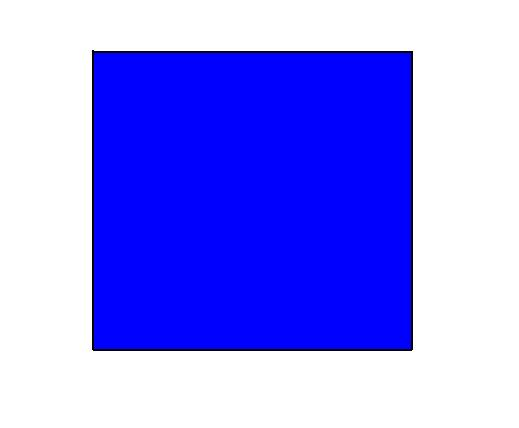
\includegraphics[width=0.30\textwidth]{./fig/quadrado}
    \label{subfig:ex2}
   }
   \caption{{\subref{subfig:ex1}} e {\subref{subfig:ex2}} representam dois exemplos do uso de subfiguras dentro de uma única figura.}
  \label{fig:subfiguras}
\fontefig{Elaborado pelo autor}
\end{figure}

A figura \ref{fig:subfiguras} foi incluída com os comandos listados a seguir. Observe que há rótulos independentes para cada uma das subfiguras e um rótulo geral para a figura, os quais podem ser todos referenciados.
\begin{Verbatim}
\begin{figure}[h]
 \centering
  \subfigure[Primeira subfigura.]
   {
    \includegraphics[width=0.35\textwidth]{./fig/exemploFig1}
    \label{subfig:ex1}
   } \qquad
  \subfigure[Segunda subfigura (um pedaço).]
   {
    \includegraphics[width=0.30\textwidth]{./fig/exemploFig2}
    \label{subfig:ex2}
   }
   \caption{{\subref{subfig:ex1}} e {\subref{subfig:ex2}} representam
             dois exemplos do uso de subfiguras dentro de uma única
             figura.}
  \label{fig:subfiguras}
  \fontefig{Elaborado pelo autor}
\end{figure}
\end{Verbatim}
 Caso uma subfiguras não tenha rótulo, para evitar que o apenas o número da mesma apareça na Lista de Figuras, use o comando \verb|\subfigure[][]|.  Caso uma subfigura tenha rótulo e deseja-se evitar que a mesma apareça na Lista de Figuras, use o comando \verb|\subfigure[][Rótulo]|.
 
 %% - - - - - - - - - - - - - - - - - - - - - - - - - - - - - - - - -
\section{Tabelas}
\label{sec:tabs} 
Em tabelas, deve-se evitar usar cor de fundo diferente do branco e o uso de linhas grossas ou duplas. Ao relatar dados empíricos, não se deve usar mais dígitos decimais do aqueles que possam ser garantidos pela sua precisão e reprodutibilidade. Rótulos de tabelas devem ser colocados
antes das mesmas (veja a Tabela \ref{tab:MarcMNem}).

\begin{table}[!ht]
\centering
\caption{Conteúdo do diretório}
\label{tab:MarcMNem} 
\begin{tabular}{c|c|c|c|c|c|c}
\hline Tag & Comprimento & Início &   & Tag & Comprimento & Início \\ 
\hline 001 & 0020 & 00000 && 100 & 0032 & 00235\\ 
\hline 003 & 0004 & 00020 && 245 & 0087 & 00267\\ 
\hline 005 & 0017 & 00024 && 246 & 0036 & 00354\\ 
\hline 008 & 0041 & 00041 && 250 & 0012 & 00390\\ 
\hline 010 & 0024 & 00082 && 260 & 0037 & 00402\\ 
\hline 020 & 0025 & 00106 && 300 & 0029 & 00439\\ 
\hline 020 & 0044 & 00131 && 500 & 0042 & 00468\\ 
\hline 040 & 0018 & 00175 && 520 & 0220 & 00510\\ 
\hline 050 & 0024 & 00193 && 650 & 0033 & 00730\\ 
\hline 082 & 0018 & 00217 && 650 & 0012 & 00763\\ 
\hline 
\end{tabular} 
\fontetab{\cite{Arm1979}}
\end{table}

% Exemplos de 2 tabelas avançadas 

\begin{table}[!ht]
\centering
\caption{Outro exemplo de tabela}
\renewcommand{\baselinestretch}{1.2}% for tabular environment
\small
\begin{tabular}{cccccc}
\hline
   & \multirow{2}{22mm}{\renewcommand{\baselinestretch}{0.7}\small\centering Quantitative measures} & \multicolumn{4}{c}{Markers} \\ \cline{3-6}
   & & \multicolumn{1}{c}{RO} & \multicolumn{1}{c}{ASF} & \multicolumn{1}{c}{ISO} & \multicolumn{1}{c}{ADF} \\ \hline
   \multirow{3}{20mm}{\renewcommand{\baselinestretch}{0.7}\small\centering Test image scale 2}
& RMSE & 0.126 & 0.187 & 0.118 & 0.103 \\
& NMSE & 0.046 & 0.101 & 0.040 & 0.031 \\
& SSIM & 0.9981 & 0.9956 & 0.9984 & 0.9989 \\ \hline
   \multirow{3}{18mm}{\renewcommand{\baselinestretch}{0.7}\small\centering Cameraman scale 4}
& RMSE & 13.748 & 15.649 & 10.132 & 4.325 \\
& NMSE & 0.011 & 0.014 & 0.006 & 0.001 \\
& SSIM & 0.923 & 0.847 & 0.904 & 0.933 \\ \hline
   \multirow{3}{18mm}{\renewcommand{\baselinestretch}{0.7}\small\centering Cameraman scale 7}
& RMSE & 20.963 & 22.652 & 13.108 & 4.650 \\
& NMSE & 0.024 & 0.029 & 0.010 & 0.001 \\
& SSIM & 0.851 & 0.757 & 0.866 & 0.925 \\ \hline
   \multirow{3}{23mm}{\renewcommand{\baselinestretch}{1.2}\small\centering Crop of cameraman scale 7}
& RMSE & 30.914 & 31.943 & 17.831 & 2.870 \\
& NMSE & 0.053 & 0.057 & 0.018 & 0.001 \\
& SSIM & 0.831 & 0.772 & 0.891 & 0.983 \\ \hline
\end{tabular}
\fontetab{Referência à fonte da tabela.}
\end{table}

\begin{table}[!ht]
\centering
\caption{Mais um exemplo de tabela}
\renewcommand{\baselinestretch}{1.2}% for tabular environment
\small
\begin{tabular}{ccccc}
\hline
\multirow{4}{16mm}{\renewcommand{\baselinestretch}{0.7}\small\centering Leveling's Scale} & \multicolumn{4}{c}{Values for the scale relation of the four different type of markers} \\ \cline{2-5}
& \multirow{3}{29mm}{\renewcommand{\baselinestretch}{1}\small\centering Structure element's size $r$ for RO and ASF} & \multicolumn{2}{c}{Isotropic diffusion} & \multirow{3}{20mm}{\renewcommand{\baselinestretch}{1}\small\centering Anisotropic diffusion iterations $t$} \\ \cline{3-4}
& & \multirow{2}{23mm}{\renewcommand{\baselinestretch}{0.7}\small\centering Standard deviation $\sigma$} & \multirow{2}{12mm}{\renewcommand{\baselinestretch}{0.7}\small\centering Kernel size} & \\
& & & & \\ \hline
1 & 1 & 0.5 & $5 \times 5$ & 100 \\
2 & 2 & 1.0 & $7 \times 7$ & 200 \\
3 & 3 & 1.5 & $11 \times 11$ & 300 \\
4 & 4 & 2.0 & $13 \times 13$ & 400 \\
5 & 5 & 2.5 & $17 \times 17$ & 500 \\
6 & 6 & 3.0 & $19 \times 19$ & 600 \\
7 & 7 & 3.5 & $23 \times 23$ & 700 \\ \hline
\end{tabular}
\fontetab{Referência à fonte da tabela.}
\end{table} 

\setlongtables
\begin{longtable}[c]{c|c|c|c|c|c}
\caption{Exemplo de tabela longa que atravessa várias páginas.}\label{tab:longas}\\
\hline
\textbf{Campo1} & \textbf{Campo2} & \textbf{Campo3} & \textbf{Campo4} & \textbf{Campo5} & \textbf{Campo6} \\
\hline\hline
\endfirsthead
\caption[]{Continuação} \\
\hline
\textbf{Campo1} & \textbf{Campo2} & \textbf{Campo3} & \textbf{Campo4} & \textbf{Campo5} & \textbf{Campo6} \\
\hline\hline
\endhead
\hline\hline
\endlastfoot
\hline
\multicolumn{6}{r}{\captionlabelfont\captionsize(Continua)}\\
\endfoot
	campo1 & campo2 & campo3 & campo4 & campo5 & campo6 \\
	campo1 & campo2 & campo3 & campo4 & campo5 & campo6 \\
	campo1 & campo2 & campo3 & campo4 & campo5 & campo6 \\
	campo1 & campo2 & campo3 & campo4 & campo5 & campo6 \\
	campo1 & campo2 & campo3 & campo4 & campo5 & campo6 \\
	campo1 & campo2 & campo3 & campo4 & campo5 & campo6 \\
	campo1 & campo2 & campo3 & campo4 & campo5 & campo6 \\
	campo1 & campo2 & campo3 & campo4 & campo5 & campo6 \\
	campo1 & campo2 & campo3 & campo4 & campo5 & campo6 \\
	campo1 & campo2 & campo3 & campo4 & campo5 & campo6 \\
	campo1 & campo2 & campo3 & campo4 & campo5 & campo6 \\
	campo1 & campo2 & campo3 & campo4 & campo5 & campo6 \\
	campo1 & campo2 & campo3 & campo4 & campo5 & campo6 \\
	campo1 & campo2 & campo3 & campo4 & campo5 & campo6 \\
	campo1 & campo2 & campo3 & campo4 & campo5 & campo6 \\
	campo1 & campo2 & campo3 & campo4 & campo5 & campo6 \\
	campo1 & campo2 & campo3 & campo4 & campo5 & campo6 \\
	campo1 & campo2 & campo3 & campo4 & campo5 & campo6 \\
	campo1 & campo2 & campo3 & campo4 & campo5 & campo6 \\
	campo1 & campo2 & campo3 & campo4 & campo5 & campo6 \\
	campo1 & campo2 & campo3 & campo4 & campo5 & campo6 \\
	campo1 & campo2 & campo3 & campo4 & campo5 & campo6 \\
	campo1 & campo2 & campo3 & campo4 & campo5 & campo6 \\
	campo1 & campo2 & campo3 & campo4 & campo5 & campo6 \\
	campo1 & campo2 & campo3 & campo4 & campo5 & campo6 \\
	campo1 & campo2 & campo3 & campo4 & campo5 & campo6 \\
	campo1 & campo2 & campo3 & campo4 & campo5 & campo6 \\
	campo1 & campo2 & campo3 & campo4 & campo5 & campo6 \\
	campo1 & campo2 & campo3 & campo4 & campo5 & campo6 \\
	campo1 & campo2 & campo3 & campo4 & campo5 & campo6 \\
	campo1 & campo2 & campo3 & campo4 & campo5 & campo6 \\
	campo1 & campo2 & campo3 & campo4 & campo5 & campo6 \\
	campo1 & campo2 & campo3 & campo4 & campo5 & campo6 \\
	campo1 & campo2 & campo3 & campo4 & campo5 & campo6 \\
	campo1 & campo2 & campo3 & campo4 & campo5 & campo6 \\
	campo1 & campo2 & campo3 & campo4 & campo5 & campo6 \\
	campo1 & campo2 & campo3 & campo4 & campo5 & campo6 \\
	campo1 & campo2 & campo3 & campo4 & campo5 & campo6 \\
	campo1 & campo2 & campo3 & campo4 & campo5 & campo6 \\
	campo1 & campo2 & campo3 & campo4 & campo5 & campo6 \\
	campo1 & campo2 & campo3 & campo4 & campo5 & campo6 \\
	campo1 & campo2 & campo3 & campo4 & campo5 & campo6 \\
	campo1 & campo2 & campo3 & campo4 & campo5 & campo6 \\
	campo1 & campo2 & campo3 & campo4 & campo5 & campo6 \\
	campo1 & campo2 & campo3 & campo4 & campo5 & campo6 \\
	campo1 & campo2 & campo3 & campo4 & campo5 & campo6 \\
	campo1 & campo2 & campo3 & campo4 & campo5 & campo6 \\
	campo1 & campo2 & campo3 & campo4 & campo5 & campo6 \\
	campo1 & campo2 & campo3 & campo4 & campo5 & campo6 \\
	campo1 & campo2 & campo3 & campo4 & campo5 & campo6 \\
	campo1 & campo2 & campo3 & campo4 & campo5 & campo6 \\
	campo1 & campo2 & campo3 & campo4 & campo5 & campo6 \\
	campo1 & campo2 & campo3 & campo4 & campo5 & campo6 \\
	campo1 & campo2 & campo3 & campo4 & campo5 & campo6 \\
	campo1 & campo2 & campo3 & campo4 & campo5 & campo6 \\
	campo1 & campo2 & campo3 & campo4 & campo5 & campo6 \\
	campo1 & campo2 & campo3 & campo4 & campo5 & campo6 \\
	campo1 & campo2 & campo3 & campo4 & campo5 & campo6 \\
	campo1 & campo2 & campo3 & campo4 & campo5 & campo6 \\
	campo1 & campo2 & campo3 & campo4 & campo5 & campo6 \\
	campo1 & campo2 & campo3 & campo4 & campo5 & campo6 \\
	campo1 & campo2 & campo3 & campo4 & campo5 & campo6 \\
	campo1 & campo2 & campo3 & campo4 & campo5 & campo6 \\
	campo1 & campo2 & campo3 & campo4 & campo5 & campo6 \\
	campo1 & campo2 & campo3 & campo4 & campo5 & campo6 \\
	campo1 & campo2 & campo3 & campo4 & campo5 & campo6 \\
	campo1 & campo2 & campo3 & campo4 & campo5 & campo6 \\
	campo1 & campo2 & campo3 & campo4 & campo5 & campo6 \\
	campo1 & campo2 & campo3 & campo4 & campo5 & campo6 \\
	campo1 & campo2 & campo3 & campo4 & campo5 & campo6 \\
	campo1 & campo2 & campo3 & campo4 & campo5 & campo6 \\
	campo1 & campo2 & campo3 & campo4 & campo5 & campo6 \\
	campo1 & campo2 & campo3 & campo4 & campo5 & campo6 \\
\hline
\end{longtable}
% o comando \fontetab{} não pode ser usado neste caso
\vspace{-8mm}
\begin{center}
\footnotesize
Fonte: Referência a fonte da tabela.
\end{center}

A \autoref{tab:longa} é um exemplo de tabela no modo paisagem e que ocupa também várias páginas.

\setlongtables
\begin{landscape}
\begin{longtable}[c]{c|c|c|c|c|c|c|c|c|c}
\caption{Exemplo de tabela longa, em paisagem, que atravessa várias páginas.}\label{tab:longa}\\
\hline
\textbf{BOX1} & \textbf{BOX2} & \textbf{BOX3} & \textbf{BOX4} & \textbf{BOX5} & \textbf{BOX6} & \textbf{BOX7} & \textbf{BOX8} & \textbf{BOX9} & \textbf{BOX10} \\
\hline\hline
\endfirsthead
\caption[]{Conclusão}\\
\hline
\textbf{BOX1} & \textbf{BOX2} & \textbf{BOX3} & \textbf{BOX4} & \textbf{BOX5} & \textbf{BOX6} & \textbf{BOX7} & \textbf{BOX8} & \textbf{BOX9} & \textbf{BOX10} \\
\hline\hline
\endhead
\endlastfoot
\hline
\multicolumn{10}{r}{\captionlabelfont\captionsize(Continua)}\\
\endfoot
	
	BOX1 & BOX2 & BOX3 & BOX4 & BOX5 & BOX6 & BOX7 & BOX8 & BOX9 & BOX10 \\
	BOX1 & BOX2 & BOX3 & BOX4 & BOX5 & BOX6 & BOX7 & BOX8 & BOX9 & BOX10 \\
	BOX1 & BOX2 & BOX3 & BOX4 & BOX5 & BOX6 & BOX7 & BOX8 & BOX9 & BOX10 \\
	BOX1 & BOX2 & BOX3 & BOX4 & BOX5 & BOX6 &	BOX7 & BOX8 & BOX9 & BOX10 \\
	BOX1 & BOX2 & BOX3 & BOX4 & BOX5 & BOX6 &	BOX7 & BOX8 & BOX9 & BOX10 \\
	BOX1 & BOX2 & BOX3 & BOX4 & BOX5 & BOX6 &	BOX7 & BOX8 & BOX9 & BOX10 \\
	BOX1 & BOX2 & BOX3 & BOX4 & BOX5 & BOX6 &	BOX7 & BOX8 & BOX9 & BOX10 \\
	BOX1 & BOX2 & BOX3 & BOX4 & BOX5 & BOX6 &	BOX7 & BOX8 & BOX9 & BOX10 \\
	BOX1 & BOX2 & BOX3 & BOX4 & BOX5 & BOX6 &	BOX7 & BOX8 & BOX9 & BOX10 \\
	BOX1 & BOX2 & BOX3 & BOX4 & BOX5 & BOX6 &	BOX7 & BOX8 & BOX9 & BOX10 \\
	BOX1 & BOX2 & BOX3 & BOX4 & BOX5 & BOX6 & BOX7 & BOX8 & BOX9 & BOX10 \\
	BOX1 & BOX2 & BOX3 & BOX4 & BOX5 & BOX6 &	BOX7 & BOX8 & BOX9 & BOX10 \\
	BOX1 & BOX2 & BOX3 & BOX4 & BOX5 & BOX6 &	BOX7 & BOX8 & BOX9 & BOX10 \\
	BOX1 & BOX2 & BOX3 & BOX4 & BOX5 & BOX6 &	BOX7 & BOX8 & BOX9 & BOX10 \\
	BOX1 & BOX2 & BOX3 & BOX4 & BOX5 & BOX6 &	BOX7 & BOX8 & BOX9 & BOX10 \\
	BOX1 & BOX2 & BOX3 & BOX4 & BOX5 & BOX6 &	BOX7 & BOX8 & BOX9 & BOX10 \\
	BOX1 & BOX2 & BOX3 & BOX4 & BOX5 & BOX6 &	BOX7 & BOX8 & BOX9 & BOX10 \\
	BOX1 & BOX2 & BOX3 & BOX4 & BOX5 & BOX6 &	BOX7 & BOX8 & BOX9 & BOX10 \\
	BOX1 & BOX2 & BOX3 & BOX4 & BOX5 & BOX6 &	BOX7 & BOX8 & BOX9 & BOX10 \\                                 
	BOX1 & BOX2 & BOX3 & BOX4 & BOX5 & BOX6 &	BOX7 & BOX8 & BOX9 & BOX10 \\
	BOX1 & BOX2 & BOX3 & BOX4 & BOX5 & BOX6 &	BOX7 & BOX8 & BOX9 & BOX10 \\
	BOX1 & BOX2 & BOX3 & BOX4 & BOX5 & BOX6 &	BOX7 & BOX8 & BOX9 & BOX10 \\
	BOX1 & BOX2 & BOX3 & BOX4 & BOX5 & BOX6 &	BOX7 & BOX8 & BOX9 & BOX10 \\
	BOX1 & BOX2 & BOX3 & BOX4 & BOX5 & BOX6 &	BOX7 & BOX8 & BOX9 & BOX10 \\
	BOX1 & BOX2 & BOX3 & BOX4 & BOX5 & BOX6 &	BOX7 & BOX8 & BOX9 & BOX10 \\
	BOX1 & BOX2 & BOX3 & BOX4 & BOX5 & BOX6 &	BOX7 & BOX8 & BOX9 & BOX10 \\
	BOX1 & BOX2 & BOX3 & BOX4 & BOX5 & BOX6 &	BOX7 & BOX8 & BOX9 & BOX10 \\
	BOX1 & BOX2 & BOX3 & BOX4 & BOX5 & BOX6 &	BOX7 & BOX8 & BOX9 & BOX10 \\
\hline
\end{longtable}
\vspace{-8mm}
% o comando \fontetab{} não pode ser usado neste caso
\begin{center}
\footnotesize
Fonte: Referência a fonte da tabela.
\end{center}
\end{landscape}

%% - - - - - - - - - - - - - - - -- - - - - - - - - - - - - - - - - -
\section{Algoritmos}
\label{sec:algor} 
Algoritmos devem ser representados no formato do Algoritmo \ref{alg:poten}, que foi descrito com o uso da classe \textsf{algorithm2e}. A rigor não é obrigatório o uso dessa classe, contudo o uso da mesma permite que seja gerada automaticamente uma lista de algoritmos logo após o sumário.

\medskip
\begin{center}
\begin{minipage}{0.92\textwidth}
\begin{algorithm2e}[H]
 \DontPrintSemicolon
 \LinesNumbered
 \SetAlgoLined
 \BlankLine
 \Entrada{vetor $A[i\,.\,.\,j]$, inteiros não negativos $i$ e $j$.}
 \Saida{vetor $A[i\,.\,.\,j]$ ordenado.}
 \BlankLine
 $n \leftarrow j - i$.\;
 \eSe{$(n<4)$}
   {Ordene com $\leq 3$ comparações.}
   {Divida $A$ em $\lceil\sqrt{n}\,\,\rceil$ subvetores de comprimento máximo $\lfloor\sqrt{n}\,\rfloor$.\;
    Aplique $MSR$ a cada um dos subvetores.\;
    Intercale os subvetores.\;}
\caption{$MSR(A,i,j)$ \label {alg:poten}}
\end{algorithm2e}
\end{minipage}
\end{center}

%% - - - - - -  - - - - - - - - - - - - - - - - - - - - - - - - - - -
\section{Códigos de Programa}
\label{sec:progs} 
Códigos de programa podem ser importados, mantendo-se a formatação original, conforme se pode ver no exemplo do Código \ref{code:prog1}. Este exemplo usa o ambiente \textsf{codigo}, definido na classe \textsf{classe-ifg}, que permite que uma lista de programas seja gerada automaticamente logo após o sumário.
\begin{center}
 \begin{codigo}[H]
   \small
   \lstinputlisting[language=Matlab]{prog/retangular.m}
   \caption{\texttt{funcao\_retangular()} }
   \label{code:prog1}
  \end{codigo}
\end{center}

%% - - - - - - - - - - - - - - - - - - - - - - - - - - - - - - - - - - -
\section{Teoremas, Corolários e Demonstrações}
\label{sec:teor}
 O uso do ambiente \textsf{theorem} permite a escrita de teoremas, como no exemplo a seguir:
\begin{verbatim}
\begin{theorem}[Pitágoras]
Em todo triângulo retângulo o quadrado do comprimento
da hipotenusa é igual a soma dos quadrados dos
comprimentos dos catetos.
\end{theorem}
\end{verbatim}

O resultado é o mostrado a seguir:

\begin{theorem}[Pitágoras]
Em todo triângulo retângulo o quadrado do comprimento da hipotenusa é igual a soma dos quadrados dos comprimentos dos catetos.
\end{theorem}

Da mesma forma pode-se usar o ambiente \textsf{proof} para demonstrações de teoremas:
\begin{verbatim}
\begin{proof}
Para demonstrar o Teorema de Pitágoras \dots
\end{proof}
\end{verbatim}

Neste caso, o resultado é:
\begin{proof}
Para demonstrar o Teorema de Pitágoras \dots
\end{proof}

Além desses dois ambientes, estão definidos os ambientes \textsf{definition} (Definição), \textsf{corollary} (Corolário), \textsf{lemma} (Lema)), \textsf{proposition} (Proposição), \textsf{comment} (Observação).

%% - - - - - - - - - - - - - -  - - - - - - - - - - - - - - - - - - -
\section{Citações Longas}
\label{sec:citacoes}

Segundo as normas da ABNT, uma citação longa (mais de 3 linhas) deve seguir uma formação especial. Para tanto foi criado o ambiente \verb|citacao|, o qual é baseado no ambiente de mesmo nome:

\begin{citacao}
Uma citação longa (mais de 3 linhas) deve vir em parágrafo separado,
com recuo de 4cm da margem esquerda, em fonte menor, sem as aspas
e com espaçamento simples.
Uma regra de como fazer citações em geral não é simples. É prudente
ler a norma da ABNT se você optar for fazer uso freqüente de citações.
Para satisfazer às exigências tipográficas que a norma pede para
citações longas, use o ambiente citacao.
\end{citacao}

Este exemplo de citação longa foi produzido com o uso do ambiente \verb|citacao|, como descrito logo a seguir:

\begin{verbatim}
\begin{citacao}
Uma citação longa (mais de 3 linhas) deve vir em parágrafo separado,
com recuo de 4cm da margem esquerda, em fonte menor, sem as aspas
e com espaçamento simples.
Uma regra de como fazer citações em geral não é simples. É prudente
ler a norma da ABNT se você optar for fazer uso freqüente de citações.
Para satisfazer às exigências tipográficas que a norma pede para
citações longas, use o ambiente citacao.
\end{verbatim}

%% - - - - - - - - - - - - - - - - - - - - - - - - - - - - - - - - -
\section{Referências e citações}

Em documentos acadêmicos podem existir as citações podem ser: \textbf{implícitas} quando as referências não fazem parte do texto ou \textbf{explícitas} quando o autor referente a citação é mencionado explicitamente na sentença. Nesse sentido, deve-se utilizar os comandos específicos para cada tipo de citação, ou seja, em citações explicitas deve-se usar o comando \verb|citeonline{}| e nas demais situações é usado o comando\verb|cite{}|. Alguns exemplos são apresentados no \autoref{qua:exemplo-citacao}.

\begin{quadro}[!ht]
\centering
\caption{Exemplos de citações no documento}
\label{qua:exemplo-citacao}
\begin{tabular}{|c|c|}        
\hline
\textbf{Código em \LaTeX} & \textbf{Código Compilado}\\ \hline\hline
\begin{minipage}[t]{8cm}
\vspace{5pt}
\begin{verbatim}
A ironia será assim uma ... proposta
por \citeonline{10520:2000:4.1-1}.
\end{verbatim}
\vspace{5pt}
\end{minipage}
&
\begin{minipage}[t]{6cm}
\vspace{5pt}
A ironia será assim uma ... proposta 
por \citeonline{10520:2000:4.1-1}.
\vspace{5pt}
\end{minipage}\\\hline

\begin{minipage}[t]{8cm}
\vspace{5pt}
\begin{verbatim}
\citeonline[p.~146]{10520:2000:4.2-2}
dizem que ... 
\end{verbatim}
\vspace{5pt}
\end{minipage}
&
\begin{minipage}[t]{6cm}
\vspace{5pt}
\citeonline[p.~146]{10520:2000:4.2-2} dizem que {...}
\vspace{5pt}
\end{minipage}\\ \hline

\begin{minipage}[t]{8cm}
\vspace{5pt}
\begin{verbatim}
``Apesar das ... da filosofia''
\cite[p.~293]{10520:2000:4.1-2}.
\end{verbatim}
\vspace{5pt}
\end{minipage}
&
\begin{minipage}[t]{6cm}
\vspace{5pt}
``Apesar das {...} da filosofia'' \cite[p.~293]{10520:2000:4.1-2}.
\vspace{5pt}
\end{minipage} \\ \hline

\begin{minipage}[t]{8cm}
\vspace{5pt}
\begin{verbatim}
Depois, ...  que prefiro
\cite{10520:2000:4.1-3}.
\end{verbatim}
\vspace{5pt}
\end{minipage}
&
\begin{minipage}[t]{6cm}
\vspace{5pt}
Depois, {...} que prefiro \cite{10520:2000:4.1-3}.
\vspace{5pt}
\end{minipage}\\ \hline
\end{tabular}
\fontequa{\cite{icmc-usp}}
\end{quadro}

Para especificar a página, seção ou capítulo consultado na referência é preciso acrescentá-lo entre colchetes com os comandos \verb|\cite[página]{}| ou \verb|\citeonline[página]{}|. O texto colocado entre colchetes aparecerá logo após o ano. Maiores informações sobre os comandos utilizados para citação posem ser consultados no manual de referência da abnTeX2, incluindo o uso de \textbf{apud} \cite{abntex2cite-alf}.

\section{Citações Indiretas}

As citações indiretas são caracterizadas como uma espécie de paráfrase das ideias de um determinado autor, ou seja, o pesquisador, por meio de suas próprias palavras, interpreta o discurso de outrem, contudo, mantendo o mesmo sentido. Outro aspecto que deve ser considerado é a necessidade de o autor (ou os autores) e o ano em que a obra foi publicada serem mencionados. 

Nas citações indiretas há duas formatações possíveis dependendo de como ocorre a citação no texto. Quando o autor é mencionado explicitamente utiliza-se o comando \verb|\citeonline{}|, caso contrário, deve utilizar o comando \verb|cite{}|. 

\section{Citações diretas}
\label{sec-citacao}

As citações diretas ocorrem quando o texto de uma referência é transcrito literalmente. As citações diretas curtas (até três linhas) são inseridas no texto entre aspas duplas. As aspas simples são utilizadas para indicar citação no interior da citação: \aspas{Nas citações, as chamadas pelo sobrenome do autor [...] incluído na sentença devem ser em letras maiúsculas e minúsculas e, quando estiverem entre parênteses, devem ser em letras maiúsculas} \cite[sec.~5]{NBR10520:2002}.

\begin{verbatim}
``Nas citações, as chamadas pelo sobrenome do autor [...] incluído na 
sentença devem ser em letras maiúsculas e minúsculas e, quando 
estiverem entre parênteses, devem ser em letras maiúsculas''
\cite[5]{NBR10520:2002}.
\end{verbatim}

Cabe ressaltar que em \LaTeX as aspas iniciais são diferentes das finais. Para tanto, pode-se utilizar o comando \verb|\aspas{CONTEUDO}| para inserir um determinado conteúdo entre aspas.

As citações diretas longas (com mais de 3 linhas) podem ser inseridas por meio do ambiente \texttt{citacao}:

\begin{citacao}
As citações diretas, no texto, com mais de três linhas, devem ser
destacadas com recuo de 4 cm da margem esquerda, com letra menor que a do texto
utilizado e sem as aspas. No caso de documentos datilografados, deve-se
observar apenas o recuo \cite[5.3]{NBR10520:2002}.
\end{citacao}

Use o ambiente assim:

\begin{verbatim}
\begin{citacao}
As citações diretas, no texto, com mais de três linhas [...] deve-se 
observar apenas o recuo \cite[5.3]{NBR10520:2002}.
\end{citacao}
\end{verbatim}

